
%(BEGIN_QUESTION)
% Copyright 2011, Tony R. Kuphaldt, released under the Creative Commons Attribution License (v 1.0)
% This means you may do almost anything with this work of mine, so long as you give me proper credit

This capacitive level sensor uses a single-wire probe as one ``plate'' of the capacitor and the metal vessel as the other ``plate'' of the capacitor:

$$\includegraphics[width=15.5cm]{i03453x01.eps}$$

Calculate the AC current through the circuit when the probe's capacitance is 385 picofarads, and also determine whether this current will {\it increase}, {\it decrease}, or {\it stay the same} as the liquid level inside the vessel goes down:

\vskip 10pt

$I$ = \underbar{\hskip 50pt}

\underbar{file i03453}
%(END_QUESTION)





%(BEGIN_ANSWER)

$I$ = \underbar{\bf 24.19} microamps, {\bf decreasing} as liquid level goes down.

\vskip 10pt

5 points for correct magnitude, 5 points for correct direction of change.

%(END_ANSWER)





%(BEGIN_NOTES)

{\bf This question is intended for exams only and not worksheets!}.

%(END_NOTES)

